\subsection{Task 3: supporting material}
\label{app:t3}
% Numbers: kode/results/task3/results.json (python run_all.py --task 3).

\begin{figure}[!htbp]
  \centering
  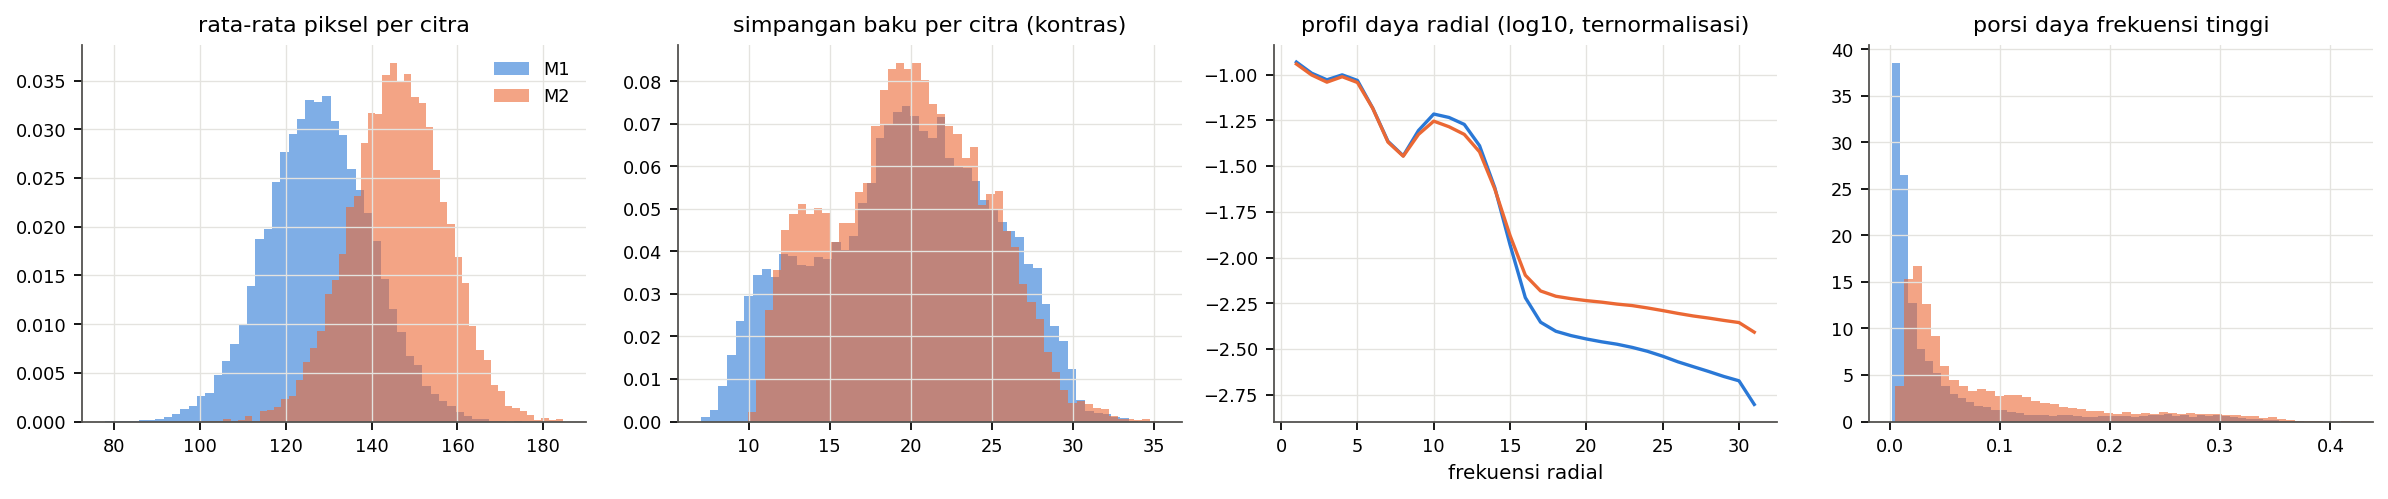
\includegraphics[width=\linewidth]{t3_eda_microscope}
  \caption{Image intensity and frequency-energy distributions across microscopes M1 and M2.}
  \label{fig:t3-eda-mic}
\end{figure}

\begin{figure}[!htbp]
  \centering
  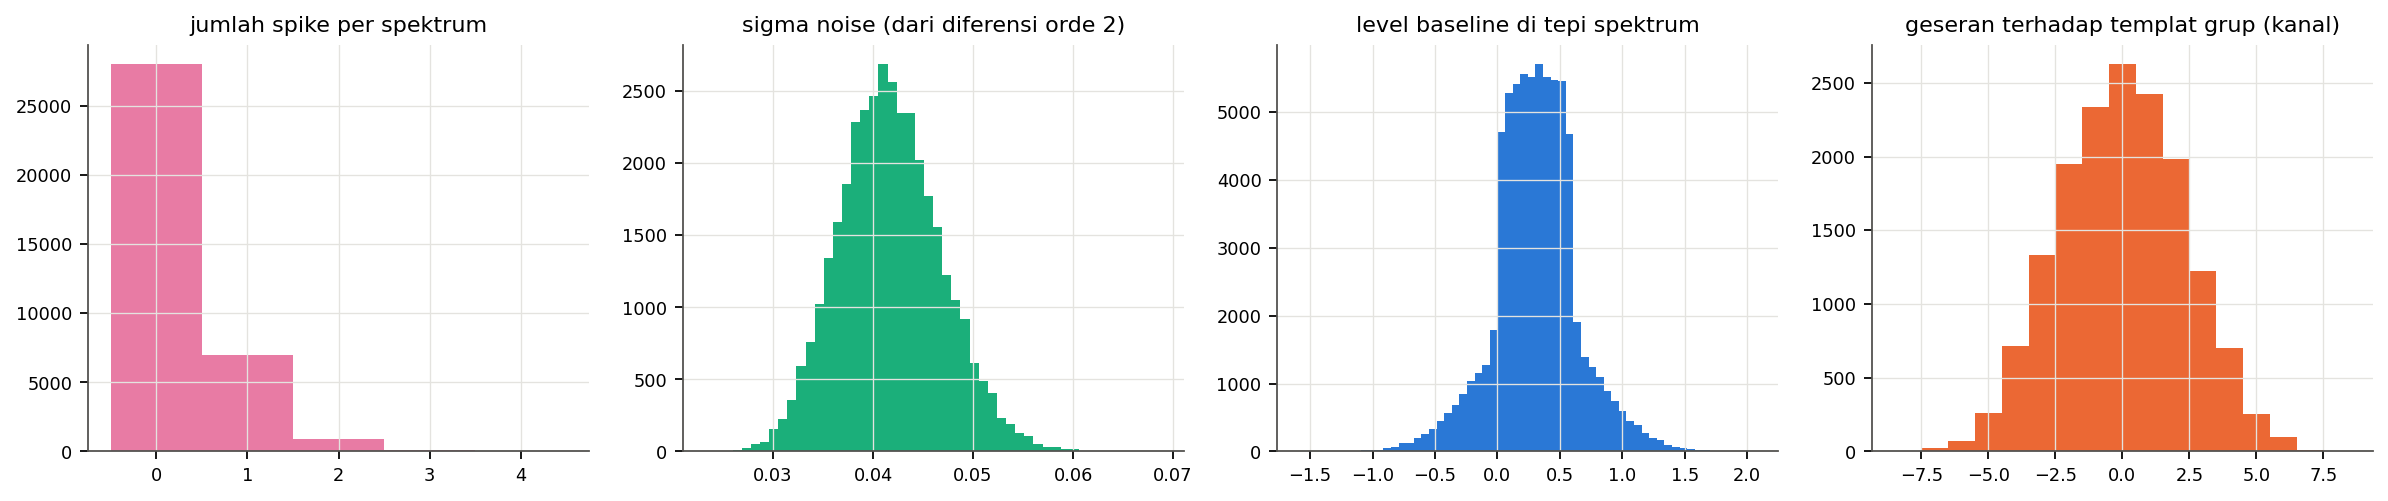
\includegraphics[width=\linewidth]{t3_eda_spectrum_distortions}
  \caption{Spectrum distortions: spikes (22.2\% of samples), baseline offset/tilt, and wavelength shift.}
  \label{fig:t3-eda-spec}
\end{figure}

\begin{figure}[!htbp]
  \centering
  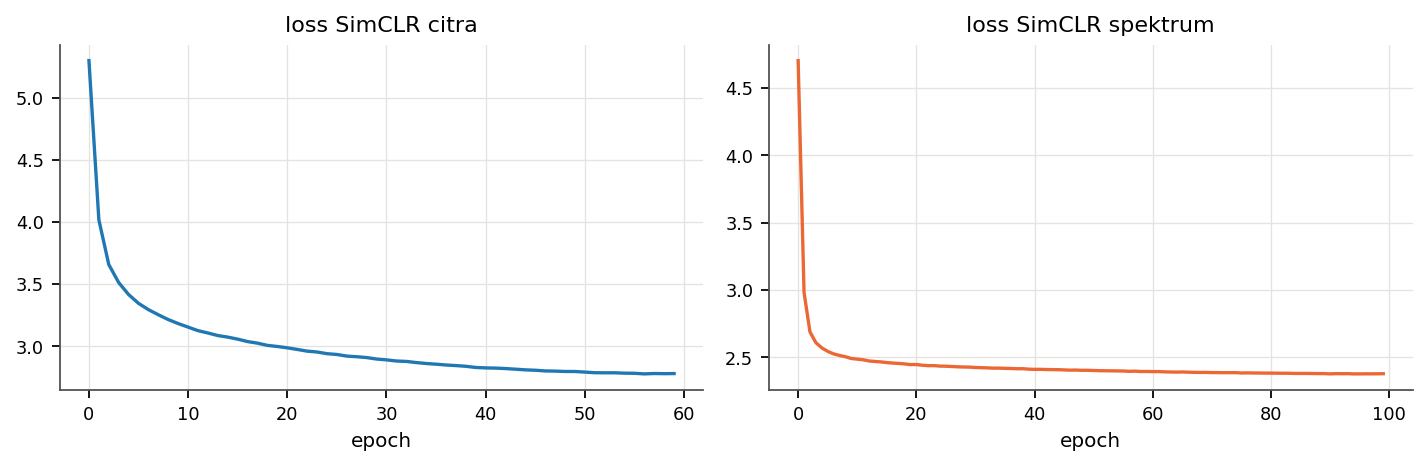
\includegraphics[width=\linewidth]{t3_simclr_loss}
  \caption{SimCLR NT-Xent training loss curves for the image (60 epochs) and spectrum (100 epochs) encoders.}
  \label{fig:t3-loss}
\end{figure}

\begin{figure}[!htbp]
  \centering
  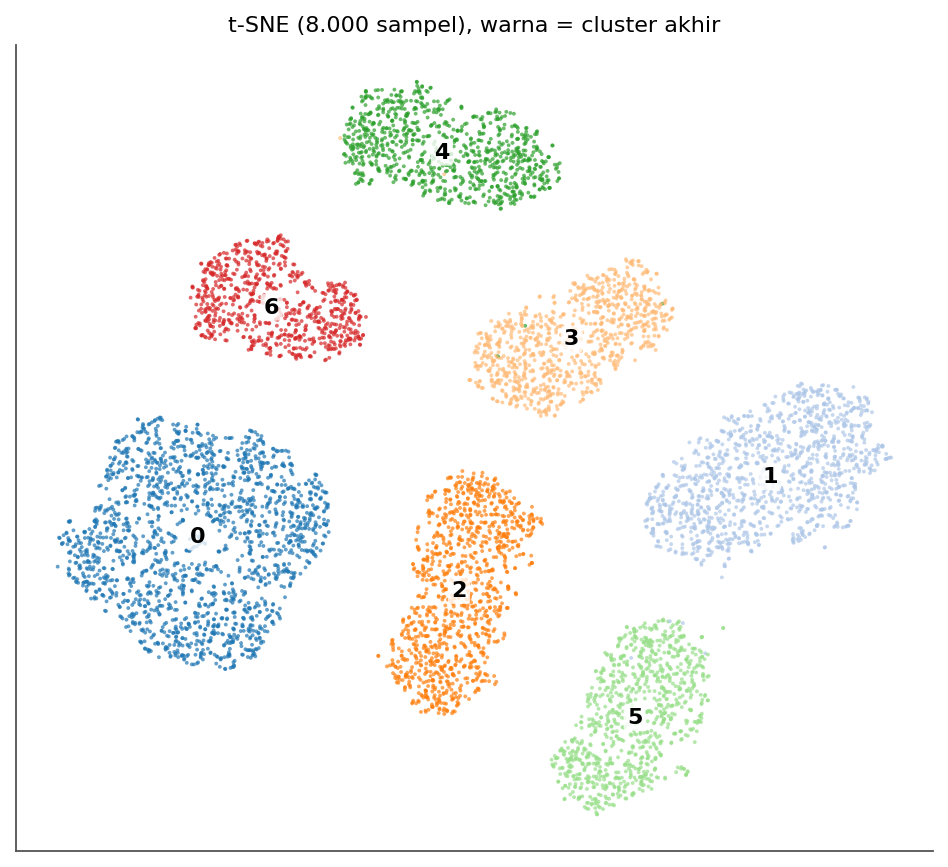
\includegraphics[width=\linewidth]{t3_tsne_clusters}
  \caption{t-SNE~\cite{vandermaaten2008tsne} projection of the fused \texttt{concat} embedding coloured by final cluster ID (0--6).}
  \label{fig:t3-tsne}
\end{figure}

\begin{figure}[!htbp]
  \centering
  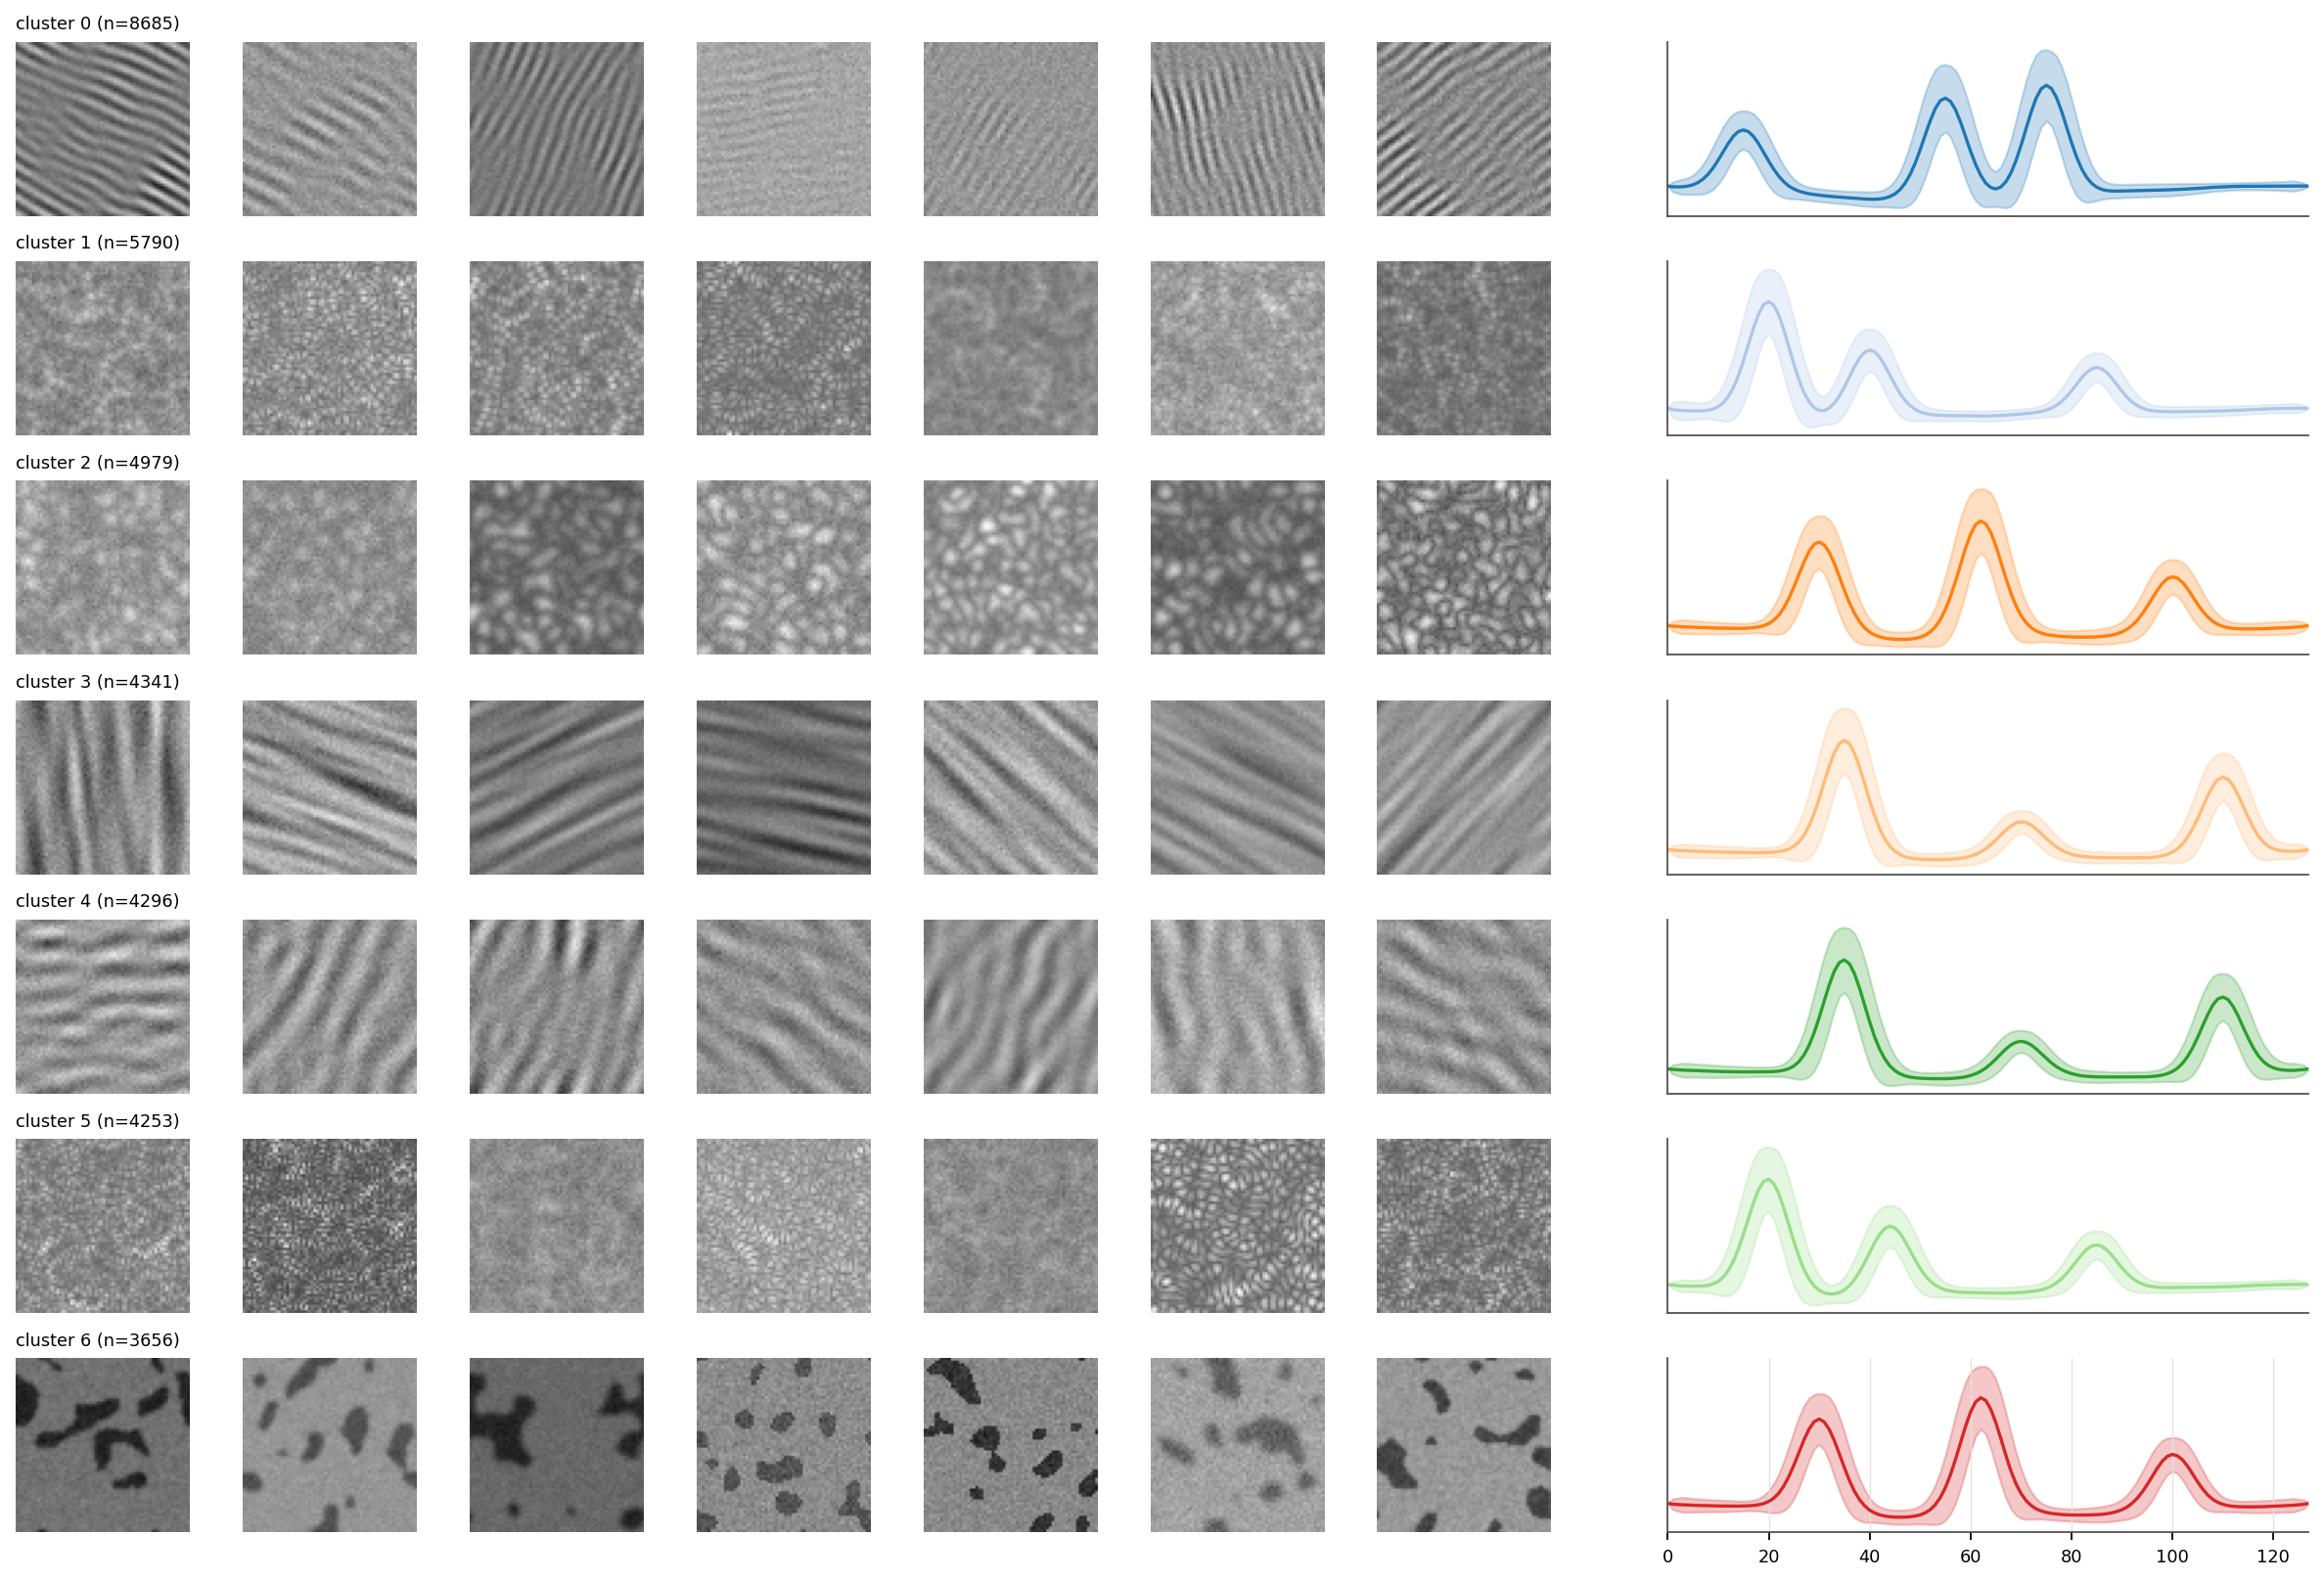
\includegraphics[width=\linewidth]{t3_cluster_profiles}
  \caption{Representative microstructure images and mean preprocessed spectra for each of the 7 clusters.}
  \label{fig:t3-profiles}
\end{figure}
